\documentclass{article}
 
\usepackage{color}
\usepackage{listings}
\usepackage{graphicx}
\usepackage{subfig}

\definecolor{MyYellow}{rgb}{1,1,0.8}
 
\lstset{language=Matlab,backgroundcolor=\color{MyYellow},basicstyle=\footnotesize,numberstyle=\footnotesize,numbers=left,stepnumber=1,numbersep=5pt,breaklines=true,frame=lines,tabsize=2}
 
\author{Ruurd Moelker \and Jan Paul Posma}
\date{\today}
\title{Signalen \& Systemen \\Practicum 3}

\begin{document}
\maketitle
 
\section{Opgave 1.1}
De filterco\"eficienten van het gezamelijke filter worden berekend door de convolutie van de twee losse filter co\"eficienten te doen volgens:
$$hh = conv([1, -2*cos(0.44*pi), 1], [1, -2*cos(0.7*pi), 1])$$
$$hh = [1, 0.8008 1.5594, 0.8008, 1]$$
De gain van het filter en de plot worden gemaakt door:
$$[H, W] = freqz( conv([1, -2*cos(0.44*pi), 1], [1, -2*cos(0.7*pi), 1]) )$$
$$plot(W/pi, abs(H));$$
De resulterende plot staat in figuur \ref{fig:opgave1_1}.

\begin{figure}[h]
	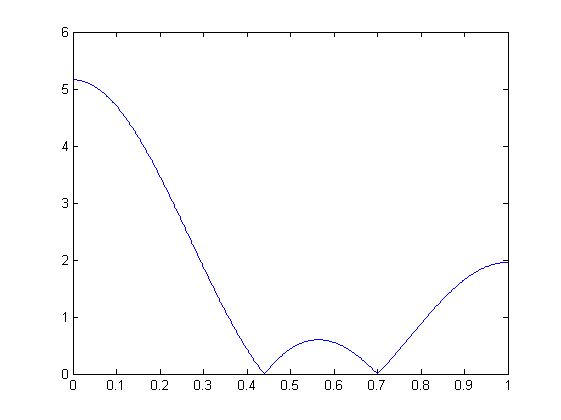
\includegraphics[width=.8\textwidth]{content/1_1.png}
	\caption{Gain filter opgave 1.1}
	\label{fig:opgave1_1}
\end{figure}

\newpage
\section{Opgave 1.2}
Het invoersignaal $x[n]$ is gemaakt met behulp van de functies:
$$nn = (0:149);$$
$$xx = 5*cos(0.3*pi*nn) + 22 * cos(0.44*pi*nn - pi/3) + 22 * cos (0.7*pi*nn - pi/4);$$


\section{Opgave 1.3}
In figuur \ref{fig:opgave1_3} staat het gefilterde signaal.

Voor $n>5$ kan het signaal gegeven worden met de functie $y = 1.9330 * 5*cos(0.3*pi*n)$, waarbij 1.9330 gevonden wordt via:
$$H = freqz(hh);$$
$$f = abs(H(floor(0.3*length(H))));$$

\begin{figure}[h]
	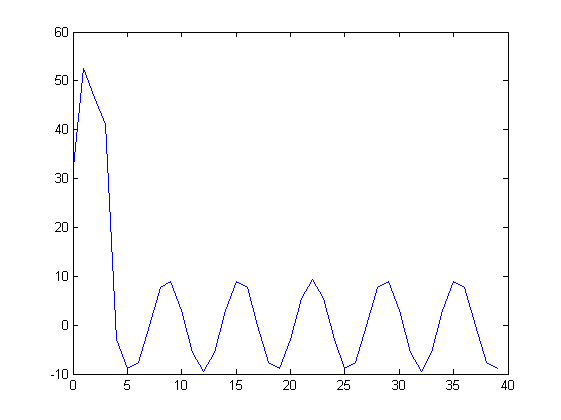
\includegraphics{content/1_3.png}
	\caption{Gain band filter}
	\label{fig:opgave1_3}
\end{figure}

\section{Opgave 1.4}
Het gefilterde signaal is de eerste 5 punten nog niet in de stable state. Daarom komt de formule niet overeen voor $n \leq 5$.

\section{Opgave 2.1}
$L = 10$
$hh2 = 2/L * cos(w*n)$ waarbij $0\leq n \leq L$

Een plot van de gain filter staat in figuur \ref{fig:opgave2_1}

De sterkte van het filter op de frequentie $0.3\pi$  = 0,28.
De sterkte van het filter op de frequentie $0.44\pi$  = 1,1.
De sterkte van het filter op de frequentie $0.7\pi$  = 0,28.

\begin{figure}[h]
	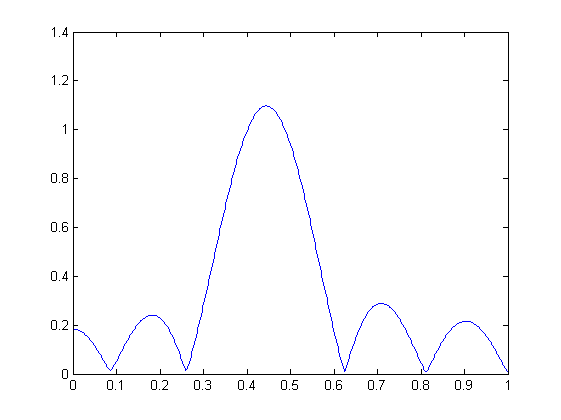
\includegraphics{content/2_1.png}
	\caption{Gain band filter}
	\label{fig:opgave2_1}
\end{figure}

\section{Opgave 2.2}

Om de frequentie waarden te vinden die in de band zitten gebruiken we voor de verschillende waarden van L achtereenvolgens:
$$nn2 = (0:19);$$
$$hh2 = 2/L* cos(W*nn2)$$
$$length(find(abs(H/max(H)) > 1/sqrt(2)))) / length(W)$$

De gevonden breedte horende bij de ingevoerde waarde van L zijn als volgt:
$$L=10 \rightarrow 0,164*pi$$
$$L=20 \rightarrow 0,086*pi$$
$$L=40 \rightarrow 0,043*pi$$


\section{Opgave 2.3}
Om de kleinste L te $\hat{\omega} = 0,44\pi$ doorlaat, maar wel de frequenties $\hat{\omega} = 0,3\pi$ en $\hat{\omega} = 0,7\pi$ sterk vermindert maken wij gebruik van een lus. De functie hieronder gebruikt een lus om de kleinste L te vinden waarvoor geldt:

\begin{list}{}{}
 \item Elke frequentiecomponent met $\hat{\omega} \leq 0,3 \pi$ wordt een factor 10 verzwakt
 \item Elke frequentiecomponent met $0,7 \pi \leq \hat{\omega} \leq \pi$ wordt met een factor 10 verzwakt
\end{list}


\begin{lstlisting}
function [L, hh] = findL( w )

L = 10;
minimumH = 0;

while (minimumH <= 0 && L < 100)
    L = L + 1;
    hh = 2/L*cos(w*(0:(L-1))); 
    H = freqz(hh);
    
    minimumLeft  = min(abs(H(1:floor(0.3*length(H)))) <= 0.1);
    minimumRight = min(abs(H(floor(0.7*length(H)) : length(H))) <= 0.1);
    minimumH = min(minimumLeft, minimumRight);
end

end
\end{lstlisting}

\section{Opgave 2.4}

Figuur \ref{fig:opgave2_4} geeft het oorspronkelijke signaal uit opgave 1.2 en het signaal gehaald door de filter uit de vorige opgaven. Deze plot is gegenereerd door de codes:
$$[L, hh] = findL(0.44*pi);$$
$$xx = 5*cos(0.3*pi*nn) + 22 * cos(0.44*pi*nn - pi/3) + 22 * cos (0.7*pi*nn - pi/4);$$
$$yy = conv(xx, hh);$$
$$subplot(2,1,1); plot((0:99), xx(1:100));$$
$$subplot(2,1,2); plot((0:99), yy(1:100));$$

Het gefilterde signaal toont maar \'e\'en frequentie heel duidelijk, namelijk $0,44 \pi$. Omdat we de frequenties onder $0,3 \pi$ en boven $0,7 \pi$ met minstens een factor 10 afzwakken, zijn die twee frequenties zelf behoorlijk afgezwakt.

%\centering
 	%\subfloat[][x[n]]{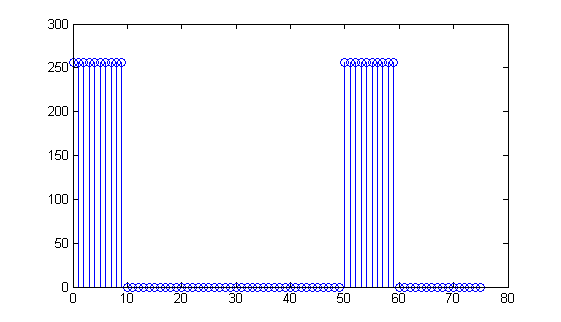
\includegraphics[width=0.4\textwidth]{content/2xx.png}}
	%\subfloat[][w[n]]{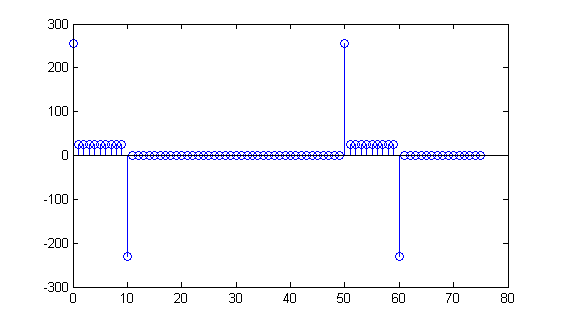
\includegraphics[width=0.4\textwidth]{content/2ww.png}}
\begin{figure}[h]
	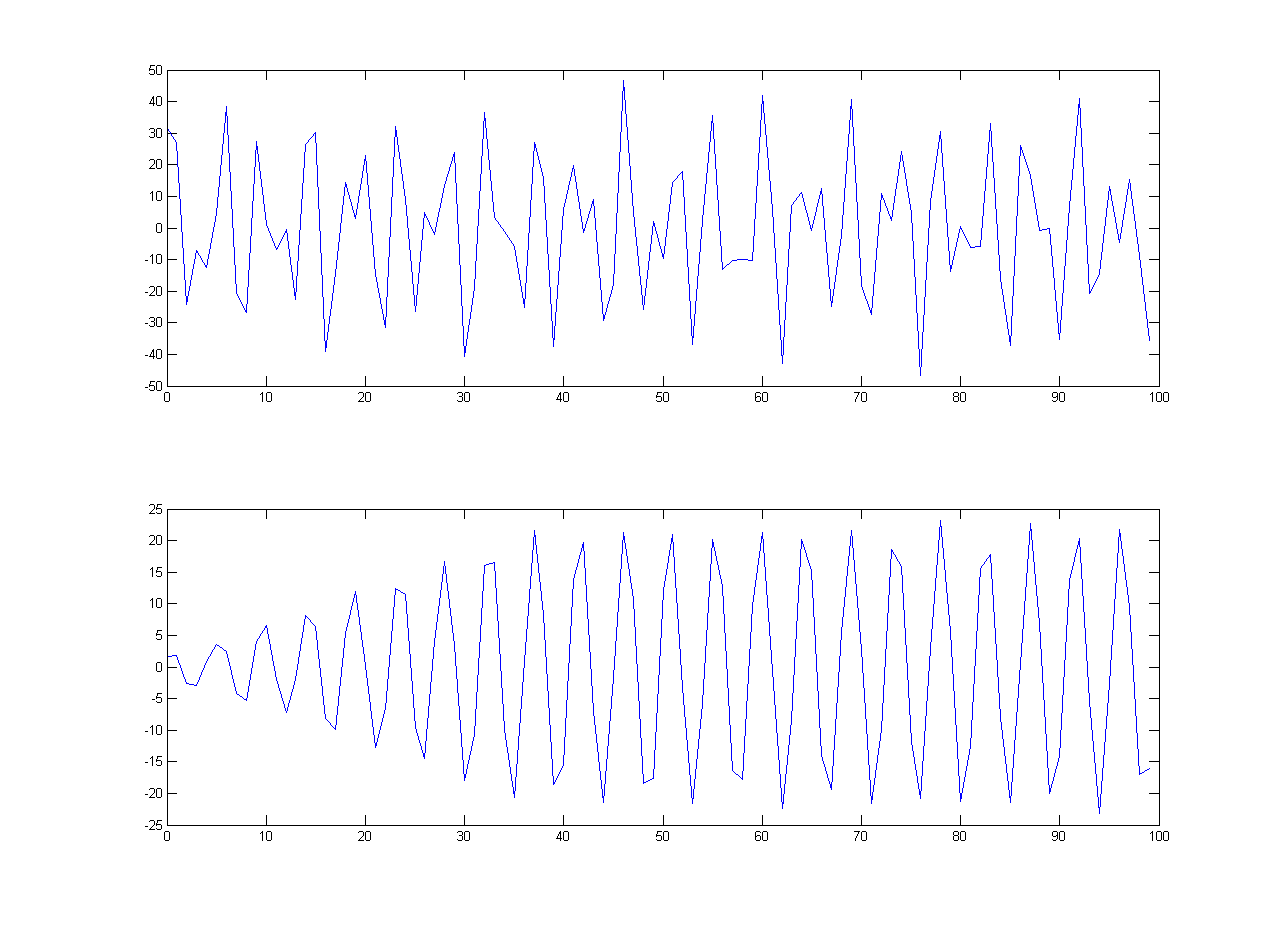
\includegraphics[width=1\textwidth]{content/2_4.png}
	\caption{Plot signaal 1.2 t.o.v. het signaal gefilterd met het systeem uit opgave 2.3}
	\label{fig:opgave2_4}
\end{figure}

\end{document}
